
\BiAppChapter{外文文献译文}{Translation}

{\centering
\vspace{-5ex}
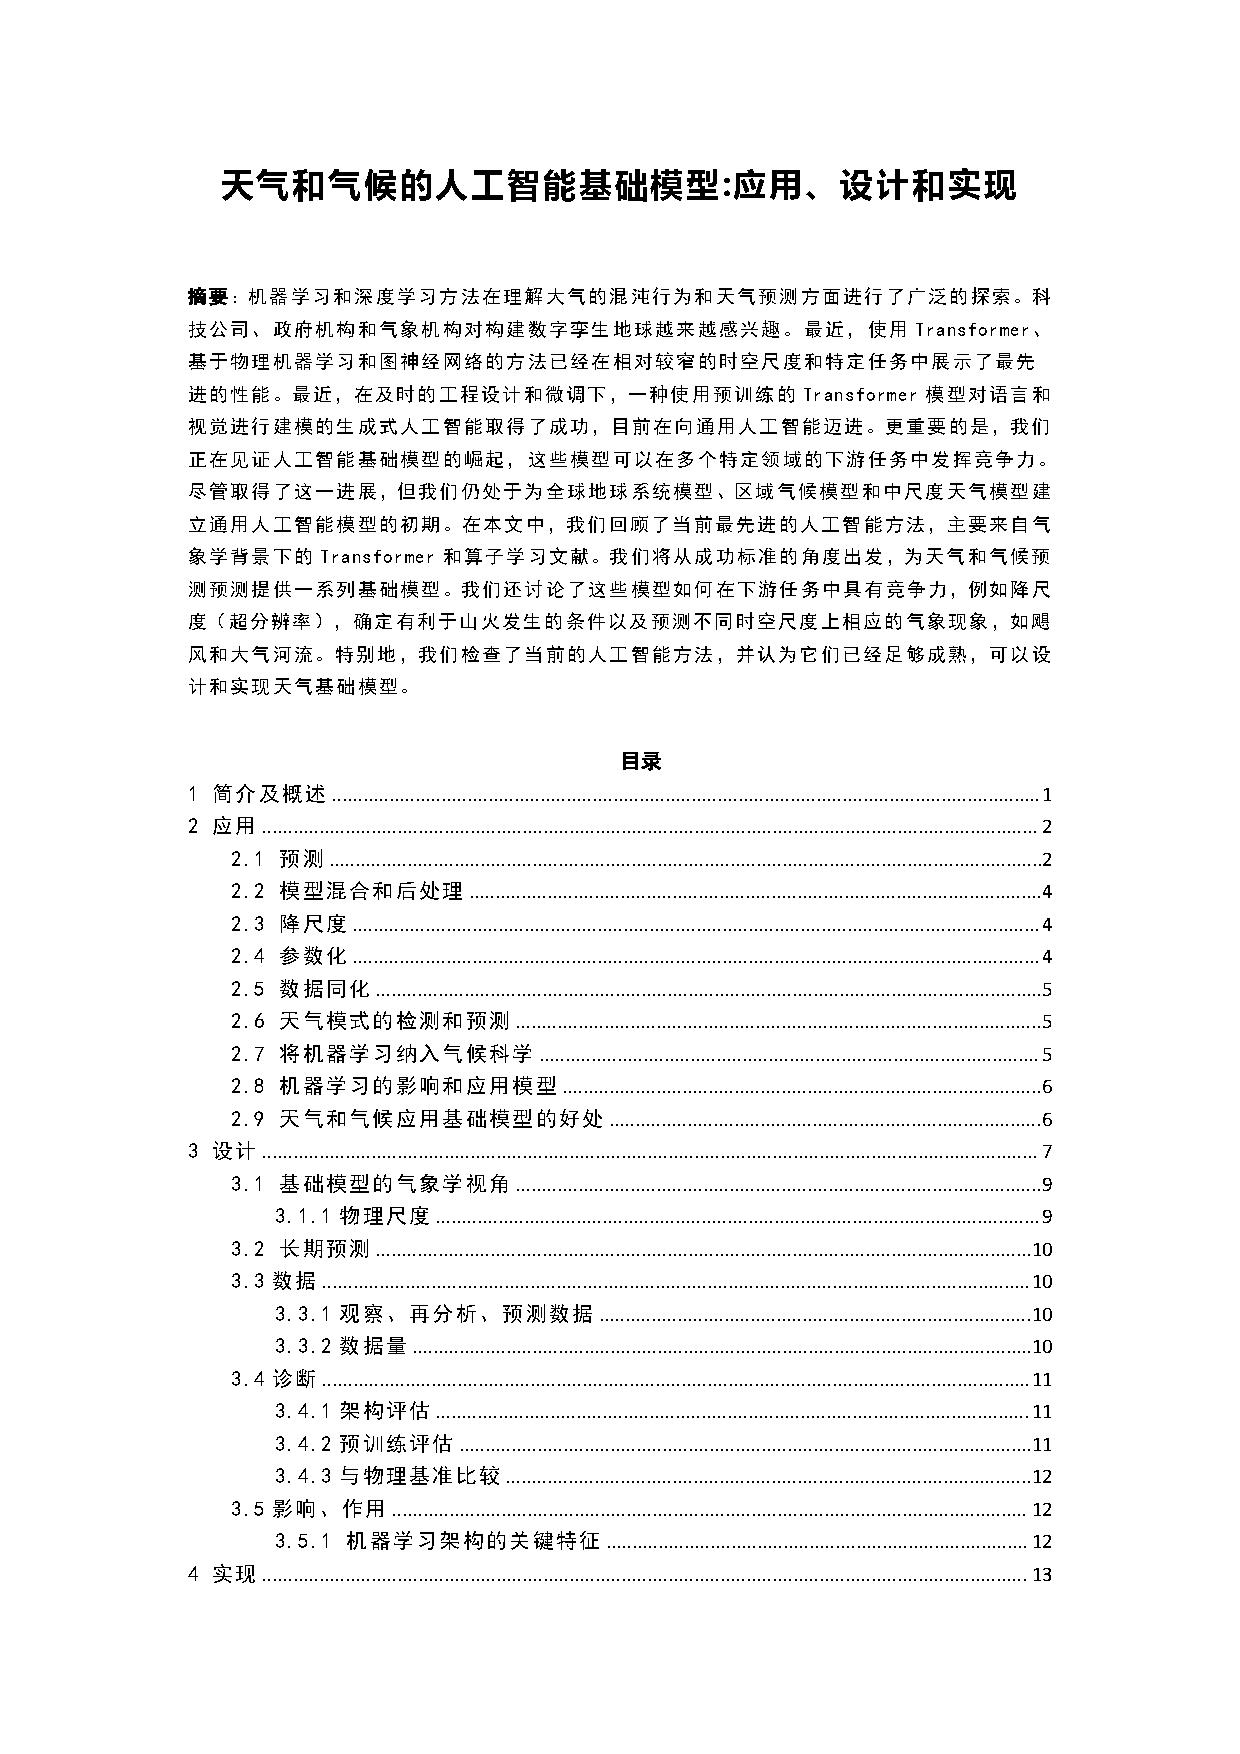
\includegraphics[width=\textwidth, page=1, trim = 15mm 20mm 15mm 20mm]{pdfs/师梓豪_2204112376_外文翻译译文.pdf}
\includegraphics[width=\textwidth, page=2, trim = 15mm 20mm 15mm 20mm]{pdfs/师梓豪_2204112376_外文翻译译文.pdf}
\includegraphics[width=\textwidth, page=3, trim = 15mm 20mm 15mm 20mm]{pdfs/师梓豪_2204112376_外文翻译译文.pdf}
\includegraphics[width=\textwidth, page=4, trim = 15mm 20mm 15mm 20mm]{pdfs/师梓豪_2204112376_外文翻译译文.pdf}
\includegraphics[width=\textwidth, page=5, trim = 15mm 20mm 15mm 20mm]{pdfs/师梓豪_2204112376_外文翻译译文.pdf}
\includegraphics[width=\textwidth, page=6, trim = 15mm 20mm 15mm 20mm]{pdfs/师梓豪_2204112376_外文翻译译文.pdf}
\includegraphics[width=\textwidth, page=7, trim = 15mm 20mm 15mm 20mm]{pdfs/师梓豪_2204112376_外文翻译译文.pdf}
\includegraphics[width=\textwidth, page=8, trim = 15mm 20mm 15mm 20mm]{pdfs/师梓豪_2204112376_外文翻译译文.pdf}
\includegraphics[width=\textwidth, page=9, trim = 15mm 20mm 15mm 20mm]{pdfs/师梓豪_2204112376_外文翻译译文.pdf}
\includegraphics[width=\textwidth, page=10, trim = 15mm 20mm 15mm 20mm]{pdfs/师梓豪_2204112376_外文翻译译文.pdf}
}

% 外文文献以图片的形式插入,不会发生失真